%\documentclass[handout]{ximera}
\documentclass[nooutcomes]{ximera}

\usepackage{gensymb}
\usepackage{tabularx}
\usepackage{mdframed}
\usepackage{pdfpages}
%\usepackage{chngcntr}

\let\problem\relax
\let\endproblem\relax

\newcommand{\property}[2]{#1#2}




\newtheoremstyle{SlantTheorem}{\topsep}{\fill}%%% space between body and thm
 {\slshape}                      %%% Thm body font
 {}                              %%% Indent amount (empty = no indent)
 {\bfseries\sffamily}            %%% Thm head font
 {}                              %%% Punctuation after thm head
 {3ex}                           %%% Space after thm head
 {\thmname{#1}\thmnumber{ #2}\thmnote{ \bfseries(#3)}} %%% Thm head spec
\theoremstyle{SlantTheorem}
\newtheorem{problem}{Problem}[]

%\counterwithin*{problem}{section}



%%%%%%%%%%%%%%%%%%%%%%%%%%%%Jenny's code%%%%%%%%%%%%%%%%%%%%

%%% Solution environment
%\newenvironment{solution}{
%\ifhandout\setbox0\vbox\bgroup\else
%\begin{trivlist}\item[\hskip \labelsep\small\itshape\bfseries Solution\hspace{2ex}]
%\par\noindent\upshape\small
%\fi}
%{\ifhandout\egroup\else
%\end{trivlist}
%\fi}
%
%
%%% instructorIntro environment
%\ifhandout
%\newenvironment{instructorIntro}[1][false]%
%{%
%\def\givenatend{\boolean{#1}}\ifthenelse{\boolean{#1}}{\begin{trivlist}\item}{\setbox0\vbox\bgroup}{}
%}
%{%
%\ifthenelse{\givenatend}{\end{trivlist}}{\egroup}{}
%}
%\else
%\newenvironment{instructorIntro}[1][false]%
%{%
%  \ifthenelse{\boolean{#1}}{\begin{trivlist}\item[\hskip \labelsep\bfseries Instructor Notes:\hspace{2ex}]}
%{\begin{trivlist}\item[\hskip \labelsep\bfseries Instructor Notes:\hspace{2ex}]}
%{}
%}
%% %% line at the bottom} 
%{\end{trivlist}\par\addvspace{.5ex}\nobreak\noindent\hung} 
%\fi
%
%


\let\instructorNotes\relax
\let\endinstructorNotes\relax
%%% instructorNotes environment
\ifhandout
\newenvironment{instructorNotes}[1][false]%
{%
\def\givenatend{\boolean{#1}}\ifthenelse{\boolean{#1}}{\begin{trivlist}\item}{\setbox0\vbox\bgroup}{}
}
{%
\ifthenelse{\givenatend}{\end{trivlist}}{\egroup}{}
}
\else
\newenvironment{instructorNotes}[1][false]%
{%
  \ifthenelse{\boolean{#1}}{\begin{trivlist}\item[\hskip \labelsep\bfseries {\Large Instructor Notes: \\} \hspace{\textwidth} ]}
{\begin{trivlist}\item[\hskip \labelsep\bfseries {\Large Instructor Notes: \\} \hspace{\textwidth} ]}
{}
}
{\end{trivlist}}
\fi


%% Suggested Timing
\newcommand{\timing}[1]{{\bf Suggested Timing: \hspace{2ex}} #1}




\hypersetup{
    colorlinks=true,       % false: boxed links; true: colored links
    linkcolor=blue,          % color of internal links (change box color with linkbordercolor)
    citecolor=green,        % color of links to bibliography
    filecolor=magenta,      % color of file links
    urlcolor=cyan           % color of external links
}

\title{More Medians}
\author{Bart Snapp and Brad Findell}

\outcome{Learning outcome goes here.}

\begin{document}
\begin{abstract}
  We think about coordinate geometry, medians, and triangles.
\end{abstract}
\maketitle

\begin{teachingnote}
Problem 1 is a good preactivity.  The centroids should all be thirds, but some students will decide they are halves.  
\end{teachingnote}
Here we use coordinates to explore several ways of thinking about the medians of triangles.  

\begin{problem}
For each set of points below, plot the points in the coordinate plane, and use a ruler to draw the triangle.  Locate the midpoint of each side, and use a ruler to draw the medians.   Check that the medians are concurrent, and find the coordinates of the centroid.  
\begin{enumerate}
\setlength{\itemsep}{4pt}
\item $A=(2, 1)$, $B=(10, 2)$, $C=(3, 6)$.  Centroid: \underline{\hspace{1.5cm}}. 
\item $D=(6, 6)$, $E=(9, 10)$, $F=(4, 8)$.  Centroid: \underline{\hspace{1.5cm}}. 
\item $G=(-1, 1)$, $H=(1, 6)$, $I=(-3, 4)$.  Centroid: \underline{\hspace{1.5cm}}. 
%\item $J=(11,-2)$, $K=(14,2)$, $L=(10, 4)$.  Centroid: \underline{\hspace{1.5cm}}. 
\end{enumerate}

\begin{image}
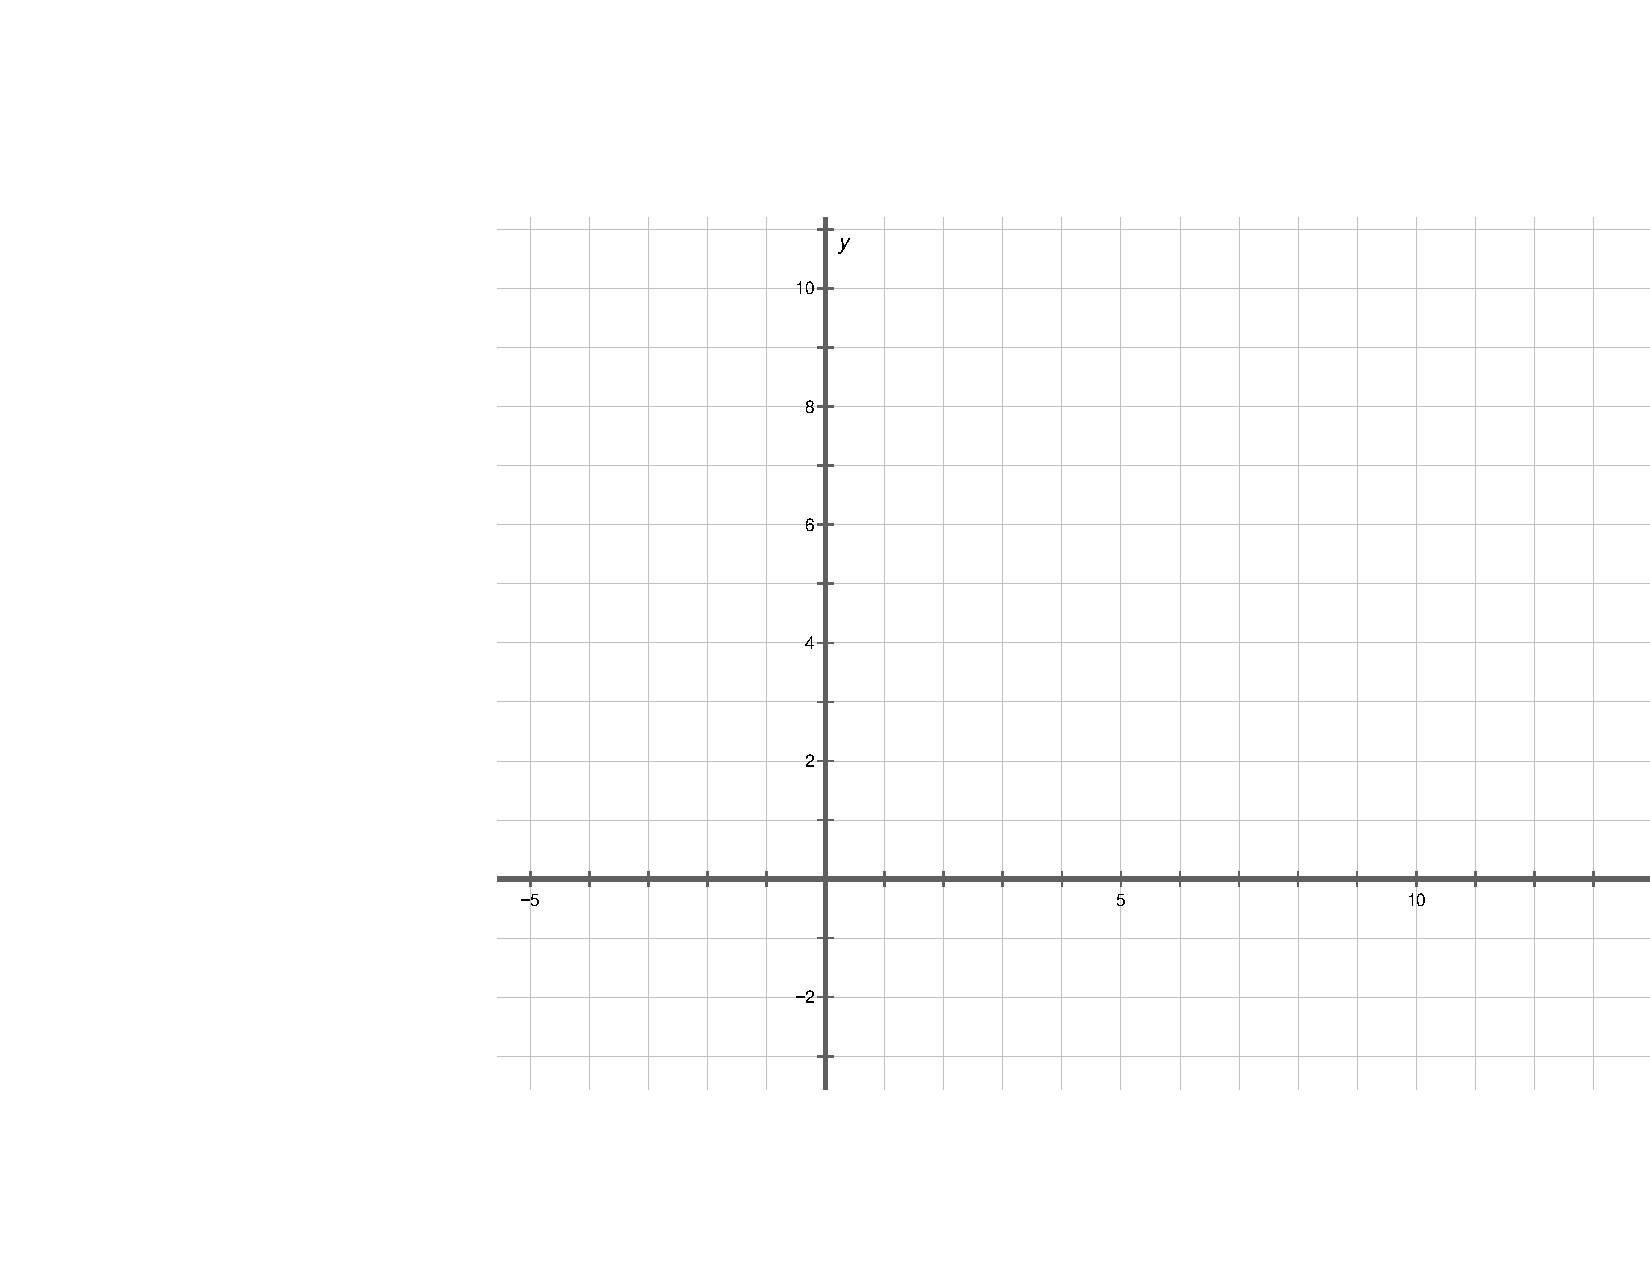
\includegraphics[width=4.5in]{graphPaper.pdf}
\end{image}

\end{problem}
\newpage

\begin{problem}
What do you notice about how the coordinates of the centroid depend upon the coordinates of the vertices?  Make a conjecture about the centroid of a triangle with vertices at $(x_1, y_1)$, $(x_2, y_2)$, and $(x_3, y_3)$.  Check that your formula works for all of the triangles above.
\vfill
\end{problem}

\begin{problem}
Imagine a triangle made of nearly weightless material with one-pound weights placed at each of the vertices, $A=(x_1, y_1)$, $B=(x_2, y_2)$, and $C=(x_3, y_3)$.  
\begin{enumerate}
\item Explain why the triangle will balance on a ruler along the median to side $\overline{AB}$.  
\vfill
\item Explain why the triangle will continue to balance along the median when the masses at $A$ and $B$ are both moved to the midpoint of $\overline{AB}$.  
\vfill
\item Now imagine trying to balance the triangle at a single point along the median.  Where will it balance?  Use the phrase ``weighted average'' to explain your reasoning.   
\vfill
\item Use weighted-average reasoning to compute the coordinates of this balance point, assuming the vertices are $A=(x_1, y_1)$, $B=(x_2, y_2)$, and $C=(x_3, y_3)$.
\vfill
\end{enumerate}
\end{problem}

\newpage
\begin{problem}
Consider a triangle with vertices at $A=(x_1, y_1)$, $B=(x_2, y_2)$, and $C=(x_3, y_3)$.  
\begin{enumerate}
\item Explain why the equation of the line containing the median from $C$ to the midpoint of $\overline{AB}$ can be written as follows:  
$$\frac{y-y_3}{x-x_3}=\frac{y_1+y_2-2y_3}{x_1+x_2-2x_3}$$
\vfill
\item From reasoning alone (i.e., without doing additional calculations) write down analogous equations for the lines containing the other two medians. 
\vfill
\item Use algebra and reasoning to show that the previously-conjectured coordinates of the centroid satisfy all three equations of lines containing medians.  
\vfill
\item Have you now proven that the medians are concurrent?  Explain.
\vfill
\end{enumerate}
\end{problem}

\end{document}
